\documentclass[]{article}


\usepackage{amsmath}
\usepackage{amssymb}
\DeclareMathOperator*{\argmax}{arg\,max}
\DeclareMathOperator*{\argmin}{arg\,min}

\usepackage{setspace}
\linespread{1.5}
\usepackage[margin=1in]{geometry}

\usepackage{graphicx}


%opening
\title{A Wasserstein-type distance in the space of Wrapped Gaussian Mixtures}
\author{Michael Wilson}
\date{}

\begin{document}
	
	\maketitle
	
	\begin{abstract}
	We present a closed form expression for the Wasserstein Distance between two Wrapped Gaussian Distributions on the sphere. We then show how to use this distance to extend some results for mixtures of Gaussians in $\mathbb{R}^d$ to mixtures of Wrapped Gaussians on the sphere. We include applications to real and simulated data. 
	\end{abstract}

\section{Introduction}

%Statistical shape analysis is a field that allows the analysis of complex, high-dimensional data sets with a non-Euclidean form of variation known as domain warping, with applications in a, b, and medical imaging. The Elastic functional data analysis framework provides a Riemannian metric in the shape space, or the quotient space of functions modulo the time-warping group. Although the shape space is a metric space, it is not a complete, separable metric space, which makes it difficult to define distributions of shapes. Usually, because distances in the shape space correspond to distances in the pre-shape space after optimal alignment, and the pre-shape space is a complete metric space, distributions of shapes are defined for aligned functions in the pre-shape space. Because the pre-shape space is a unit sphere, one can compare shape distributions in this way by comparing distributions of optimally aligned functions on the unit sphere. 
%
%Still, this does not solve the problem of how to compare these distributions on the sphere. The approach of this paper is to compare distributions of shapes by approximating the distributions as (possibly uni-modal) Wrapped Gaussian mixtures, and then calculating a Wasserstein-type distance between them. For Gaussian distributions, a closed form solution for the Wasserstein distance is available, with a similar result holding for Wrapped Gaussian distributions on non-linear manifolds, such as the sphere. By combining a Wasserstein-type distance based on this closed form solution with the theory necessary for extending it to the sphere yields a computationally simple method for calculating Wasserstein-type distances between Gaussian mixture distributions of shapes.    

The paper proceeds as follows; in section \ref{section: theory}, we cover background information on Wrapped Normal Distributions and Wrapped Gaussian mixtures on the sphere, Optimal Transport and the Wasserstein distance, and Wasserstein-type distances for Gaussian mixtures. In section \ref{section: wrapped gaussian mixture wasserstein-type distance}, we present a closed form expression for a Wasserstein-type distance for wrapped Gaussian mixtures on the sphere. In section \ref{section: implementation}, we present our computational implementation for calculating the Wasserstein-type distance for wrapped Gaussian mixtures on the sphere, and in section \ref{section: applications} we show applications for real and simulated data. Section \ref{section: conclusion} concludes.  

\section{Background}\label{section: theory}

%Let $\mu = \mathcal{WN}(m,\Sigma)$ be a wrapped normal distribution defined on the $d-1$ dimensional sphere $S^{d-1}$. We can define the density of $\mu$ in terms of the tangent space $T_m(S_{d-1})$, with orthonormal basis B as; 
%
%\begin{equation*}
%	\rho_\mu(x) = det(2 \gamma \Sigma) exp(-\frac{1}{2} \langle B Exp_m^{-1}(x), \Sigma^{-1} B Exp_m^{-1}(x) \rangle) 
%\end{equation*}
%
%Here $exp$ corresponds to the exponential function, while $Exp$ corresponds to the Exponential Map for $S^{d-1}$.

%\subsection{Function Registration with the Fisher-Rao Metric}
%
%We provide a brief introduction to Function Registration with the Fisher-Rao metric. For the complete details, see \cite{https://doi.org/10.48550/arxiv.1103.3817}.
%
%Let $\mathcal{F} = \{ f \in \mathbb{L}^2([0,1], \mathbb{R}): f \text{ abs. cont.}\}$. For each $f \in \mathcal{F}$, define its square-root velocity function (SRVF) representation to be $q(t) = \dot{f}(t)/\sqrt{\dot{f}(t)}$. %The absolute continuity of $f$ guarantees that its corresponding SRVF is square integrable. 
%One nice property of the SRVF transformation is that the (parameterization invariant) Fisher-Rao distance between two absolutely continuous functions is equal to the $\mathbb{L}^2$ distance between their corresponding SRVF's;
%
%\begin{equation*}
%	d_{FR}(f_1,f_2) = \sqrt{\int_0^1 (q_1(t) - q_2(t))^2 dt} = ||q_1 - q_2|| 
%\end{equation*}
%
%We refer to the set of absolutely continuous functions as $\mathcal{F}$, and the set of SRVF's as $\mathbb{L}^2$. Now, consider the time-warping group $\Gamma = \{\gamma: [0,1] \to [0,1], \gamma(0) = 0, \gamma(1) = 1, \gamma \text{ diffeo}\}$. Most approaches to function registration seek to align functions by solving $\inf_{\gamma \in \Gamma} ||f_1 - f_2 \circ \gamma||$. However, this formulation is not symmetric (and thus does not define a proper distance), and leads to alignments that 'pinch' and 'tear' the functions being aligned. By aligning functions with respect to the Fisher-Rao metric, that is, by instead focusing on the problem $\inf_{\gamma \in \Gamma} d_{FR}(f_1,f_2 \circ \gamma)$, one finds a time-warping distance that is a Riemannian metric, due to the parameterization invariance of the Fisher-Rao metric. 
%
%To see this, we note that, by an application of the chain-rule, the SRVF of $f(\gamma(t))$ is $q(\gamma(t))\sqrt{\dot{\gamma}(t)}$, and thus defining the group action of $\Gamma$ on $\mathbb{L}^2$ to be $q * \gamma = q(\gamma(t))\sqrt{\dot{\gamma}(t)}$, we have that
%
%    \begin{equation*}
%    	\inf_{\gamma \in \Gamma} d_{FR}(f_1 \circ \gamma, f_2) = \inf_{\gamma \in \Gamma} ||q_1 * \gamma - q_2||
%    \end{equation*}
%
%Because $\Gamma$ is a group, we can define the orbit of an SRVF $q \in \mathbb{L}^2$ to be $[q] = closure(\{q * \gamma : \gamma \in \Gamma \})$, referred to as a 'shape orbit', and define the shape space $\mathcal{S}$ to be the set of all such shape orbits. Thus, defining
%
%\begin{equation}
%	d_\mathcal{S}([q_1],[q_2]) = \inf_{\gamma \in \Gamma} ||q_1 - q_2 * \gamma||
%\end{equation}      
%
%it can be shown that $(\mathcal{S},d_\mathcal{S})$ is a metric space.
%
%\subsubsection{Pre-shape space}
%
%While $(\mathcal{S},d_\mathcal{S})$ is a metric space, because it is not a complete, seperable metric space, it is generally not possible to model distributions of shapes in the shape space with the distributions commonly used in statistics. Typically, to get around this, one defines distributions over the 'pre-shape' space between optimally aligned functions.   
%
%For the SRVF representation of absolutely continuous functions, the pre-shape space corresponds to the set of norm 1 SRVF's, or in other words, the unit sphere in $\mathbb{L}^2$. By taking a set of SRVF's, and optimally aligning them to their Karcher mean, one can define distributions in the pre-shape space that preserve the shape distances of each aligned SRVF to their shape mean. Because the pre-shape space can be seen as a push-forward of $\mathbb{R}^d$, we can model shape distributions as 'wrapped' versions of any distribution that can be defined over $\mathbb{R}^d$. For a set of SRVF's $Q = \{q_i \in \mathbb{L}^2, i = 1,...,n\}$, we can map them to their pre-shape representation by dividing them by their norm; $P = \{p_i = \frac{q_i}{||q_i||} \in Q, i = 1,...,n\}$. Defining $\mu$ to be the Karcher mean of the $p_i$'s, we can define the optimally aligned pre-shapes as $\{p_i * \gamma_i, i = 1,...,n\}$, where $\gamma_i = \inf_{\gamma \in \Gamma} ||p_i*\gamma - \mu||$.
%
%Thus, to represent a distribution of shapes 
%
%%Furthermore, because optimally aligned SRVF's are closed under convex combination, these distributions in the pre-shape space are consistent with distributions over the shape at least over the convex hull of the optimally aligned functions. 
%%
%Thus, to compare the distributions of two sets of shapes, one can compare their corresponding distributions in the pre-shape space. 

\subsection{Wrapped Normal Distributions and Wrapped Gaussian Mixtures on the sphere}

\subsection{Optimal Transport/ Wasserstein distances}

The Wasserstein distance is a distance between probability measures. 

\begin{equation}
	W_2^2(\mu_0, \mu_1) = \inf_{\gamma \in \Pi(\mu_0, \mu_1)} \int_{\mathcal{X}\times\mathcal{Y}} ||x - y|| d\gamma(x,y)
\end{equation}

\subsection{Wasserstein and Wasserstein-type distances for Gaussians and Wrapped Gaussians}

\section{A Wasserstein-type Distance for Wrapped Gaussian Mixtures}\label{section: wrapped gaussian mixture wasserstein-type distance}


Let $\mu_i = N(0,\Sigma_i$), $i = \{0,1\}$ be Gaussian distributions defined on $\mathbb{R}^{d-1}$, with random variables $X_i \sim \mu_i$. For some $m_i \in S^{d-1}$, let $\tilde{\mu}_i = Exp(m_i)_\#\mu_i$, (and thus $\tilde{\mu}_i = WN(m_i, \Sigma_i)$)   and let $\tilde{X}_i \sim \tilde{\mu}_i$. Then, 


\begin{equation*}
	W_2^2(\tilde{\mu_0},\tilde{\mu_1}) = cos^{-1}( \langle m_0, m_1 \rangle ) + tr(\Sigma_0 + \Sigma_1 - 2(\Sigma_0^{\frac{1}{2}}\Sigma_1\Sigma_0^{\frac{1}{2}})^{\frac{1}{2}})
\end{equation*} 

To establish our next result, it is important to note that the optimal coupling is also a wrapped Gaussian. Both of the above facts are proved in \cite{WGOT}.


%\textbf{Proof:}
%
%Let $\tilde{X} = \tilde{X}_0$ and $\tilde{Y} = Exp_{m_0}(R_\alpha(Exp_{m_1}^{-1}(\tilde{X}_1)))$. Then,
%
%
%
%\begin{equation*}
%	W_2^2(\tilde{\mu}_0, \tilde{\mu}_1) =  \inf_{\gamma \in \Pi(\tilde{\mu}_0, \tilde{\mu}_1)} \int_{TS^{d-1}} cos^{-1}(\langle \tilde{x}, \tilde{y} \rangle) \ d\tilde{\gamma}(\tilde{x},\tilde{y})
%\end{equation*}  
%
%\begin{equation}
%	=  d_{S^{d-1}}^2(E\tilde{X}_1, E\tilde{X}_2) + \inf_{\gamma \in \Pi(\tilde{\mu}_0, \tilde{\mu}_1)}\int_{T_{m_0}(S^{d-1})} \sqrt{\langle Exp_{m_0}^{-1}(\tilde{x}) - R_\alpha(Exp_{m_1}^{-1}(\tilde{y}), Exp_{m_0}^{-1}(\tilde{x}) - R_\alpha(Exp_{m_1}^{-1}(\tilde{y})) \rangle} \ d\tilde{\gamma}(\tilde{x},\tilde{y})
%\end{equation}
%
%\begin{equation}
%	= cos^{-1}( \langle m_0, m_1 \rangle ) +\inf_{\gamma \in \Pi({\mu}_0, {\mu}_1)} \int_{\mathbb{R}^{d-1} \times \mathbb{R}^{d-1}} \sqrt{ \langle x - y, x-y\rangle} \ d\gamma(x,y)
%\end{equation} 
%
%\begin{equation*}
%	= cos^{-1}( \langle m_0, m_1 \rangle ) + tr(\Sigma_0 + \Sigma_1 - 2(\Sigma_0^{\frac{1}{2}}\Sigma_1\Sigma_0^{\frac{1}{2}})^{\frac{1}{2}})
%\end{equation*} 
%
%Where the equality in equation 1 follows from Proposition 2 in \cite{WGOT}, using $m_0$ as $p_{ref}$, and the equality in equation 2 holds since $\forall \gamma \in \Pi(\mu_0, \mu_1)$, if $\tilde{\gamma} = {Exp(m_0,m_1)}_\# \gamma$ we have that 
%
%%\begin{equation*}
%%	E||\tilde{X}-\tilde{Y}||  
%%\end{equation*}  
%
%\begin{equation*}
%	= \int_{TS^{d-1}} cos^{-1}(\langle \tilde{x}, \tilde{y} \rangle) \ d\tilde{\gamma}(\tilde{x},\tilde{y})
%\end{equation*}
%
%\begin{equation*}
%	= \int_{S^{d-1}\times S^{d-1}} \sqrt{\langle Exp_{m_0}^{-1}(\tilde{x}) - R_\alpha(Exp_{m_1}^{-1}(\tilde{y}), Exp_{m_0}^{-1}(\tilde{x}) - R_\alpha(Exp_{m_1}^{-1}(\tilde{y})) \rangle} \ d\tilde{\gamma}(\tilde{x},\tilde{y})
%\end{equation*}
%
%%\begin{equation*}
%%	= \int_{\mathbb{R}^{d-1} \times \mathbb{R}^{d-1}} \sqrt{\langle Exp_{m}^{-1}(Exp_{m}(x)) - Exp_{m}^{-1}(Exp_{m}(y)), Exp_{m}^{-1}(\tilde{x}) - Exp_{m}^{-1}(\tilde{y}) \rangle} \ d\gamma({x},{y})
%%\end{equation*}
%
%\begin{equation*}
%	= \int_{\mathbb{R}^{d-1} \times \mathbb{R}^{d-1}} \sqrt{ \langle x - y, x-y\rangle} \ d\gamma(x,y)
%\end{equation*}
%
%%\begin{equation*}
%%	= E||{X}-{Y}||  
%%\end{equation*}  
%
%\begin{equation}
%	\implies \inf_{\gamma \in \Pi(\tilde{\mu}_0, \tilde{\mu}_1)} \int_{TS^{d-1}} cos^{-1}(\langle \tilde{x}, \tilde{y} \rangle) \ d\tilde{\gamma}(\tilde{x},\tilde{y}) = \inf_{\gamma \in \Pi({\mu}_0, {\mu}_1)} \int_{\mathbb{R}^{d-1} \times \mathbb{R}^{d-1}} \sqrt{ \langle x - y, x-y\rangle} \ d\gamma(x,y)
%\end{equation}  
%
%
%Furthermore, because we know that the optimal coupling in the Euclidian case is a Normal distribution, we see that the optimal coupling in the spherical case is therefore a wrapped Gaussian distribution. 

\subsection{Wrapped Gaussian Mixture Wasserstein-type Distance}

Our proof is identical to the one presented in section 4.2 of \cite{https://doi.org/10.48550/arxiv.1907.05254}, except replacing their $W_2^2$ with our $W_2^2$, and their $GMM(*)$ with our $WGMM(*)$. 


\newpage

\section{Computational Details}\label{section: implementation}

\subsection{Wrapped Gaussian Wasserstein Distance}

Let $\mu_i = WN(m_i,\Sigma_i)$, $i = \{0, 1\}$. Let $U_0 S_0 U_0^t$ denote the SVD of $\Sigma_0$, with $u_j$ the jth row of $U_0$. Define $\Sigma_0^* = U_0^* S_0 U_0^{*t}$, where the jth row of $U_0^*$ is the parallel transport of $u_j$ from $T_{m_0}(S^d)$ to $T_{m_1}(S^d)$;

%Define $\tilde{X}_i = Exp_{m_0}^{-1}(X_i)$, $\tilde{Y}_i = Exp_{m_1}^{-1}(Y_i)$, where;
%
%\begin{equation}
%	Exp_{p}^{-1}(q) = \frac{\theta}{\sin(\theta)}(q - cos(\theta)p), \text{ where } \theta = cos^{-1}(\langle p,q \rangle)  
%\end{equation} 

\begin{equation*}
	u_j^{*} = u_j - (2(u_j*m_1^t)(|m_0 +m_1|^2))(m_0 + m_1)
\end{equation*} 

Then 

\begin{equation*}
	W_2^2(\mu_0,\mu_1) = cos^{-1}(\langle m_0,m_1 \rangle) + tr(\Sigma_0^* + \Sigma_1 - 2 (\Sigma_0^{*\frac{1}{2}} \Sigma_1 \Sigma_0^{*\frac{1}{2}})^{\frac{1}{2}}) 
\end{equation*}

\subsection{Wrapped Gaussian Mixture Wasserstein-like Distance}

Let $\mu_i = \Sigma_{k=1}^{K_i} \frac{w_{ik}}{\Sigma_k w_{ik}}WN(m_{ik},\Sigma_{ik})$, $i = \{0, 1\}$, be two wrapped Gaussian mixtures. Let $\Pi(w_0, w_1) = \{ W \in \mathbb{R}^{K_0 \times K_1}, \Sigma_i W_{ij} = w_{1i},\Sigma_j W_{ij} = w_{0j}\}$. Then,

%Let $w^*$ be a solution of the discrete linear program
%
%\begin{equation}
%	\underset{w \in \Pi(w_0,w_1)}{\inf} \underset{{\ell, k}}{\Sigma} w_{\ell k} W_2^2(\mu_0^\ell,\mu_1^k)
%\end{equation} 
%
%Then,

\begin{equation}\label{eq: mixture distance}
	WMW_2^2(\mu_0,\mu_1) = \underset{W \in \Pi(w_0,w_1)}{\min}  \underset{{\ell, k}}{\Sigma} W_{\ell k} W_2^2(\mu_0^\ell,\mu_1^k)
\end{equation} 

where the minimization is performed with linear programming. 

\section{Applications}\label{section: applications}

\subsection{Simulated data}

We present plots of simulated Wrapped Gaussian Mixtures on the sphere, and include the distance calculated. 

\begin{figure}
		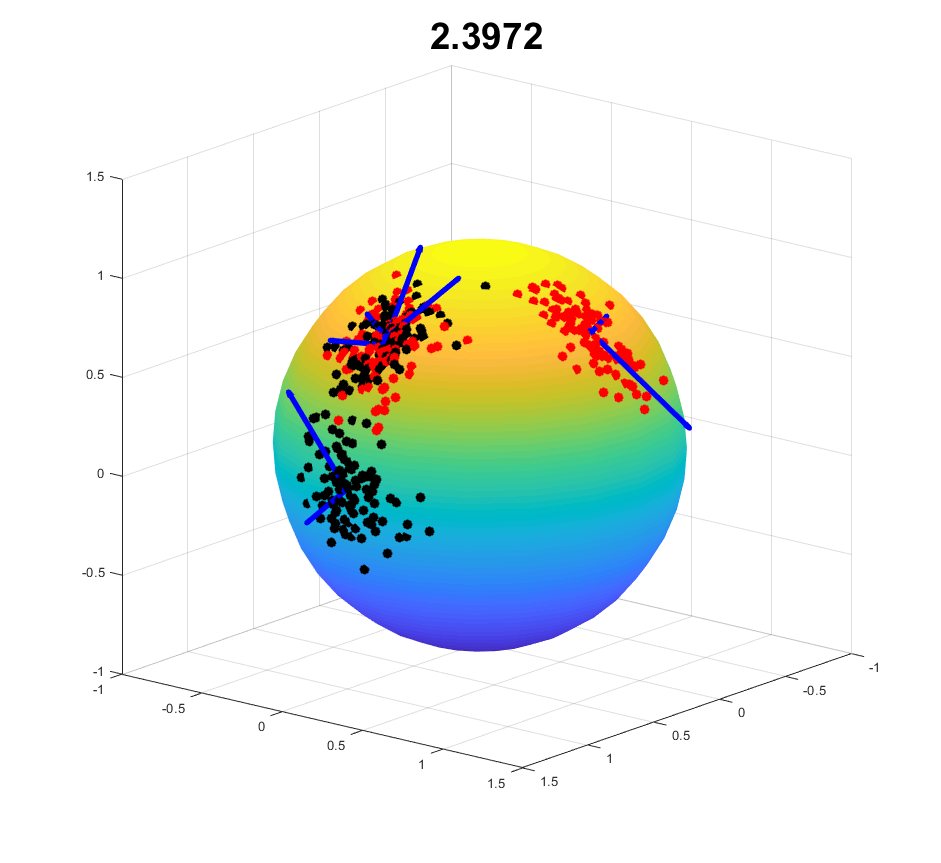
\includegraphics[width=.3\linewidth]{example6.png}
		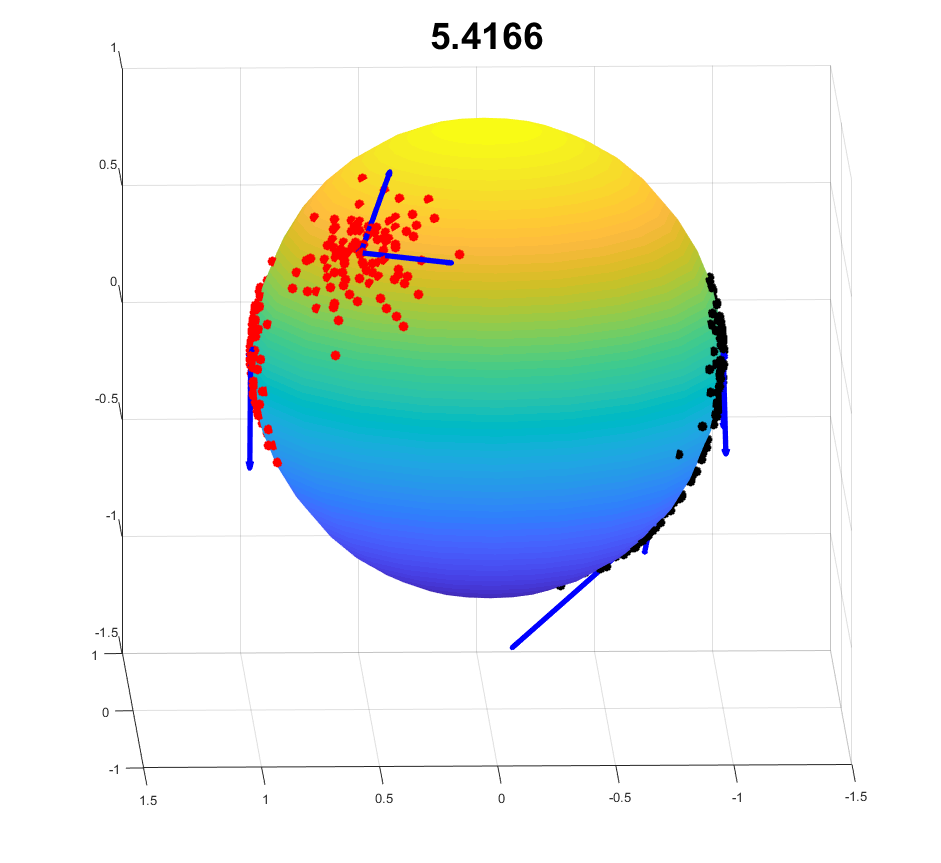
\includegraphics[width=.3\linewidth]{example8.png}
		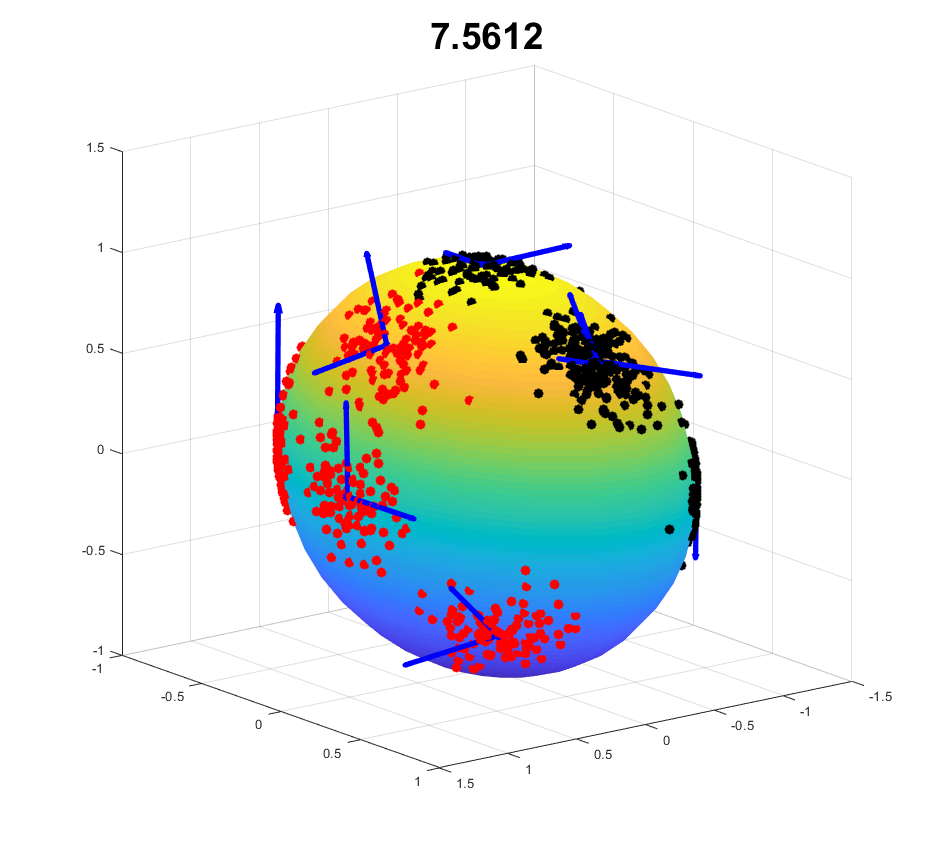
\includegraphics[width=.3\linewidth]{example10.png}
		\caption{Examples of Wrapped Gaussian Mixture Wasserstein-type distances on the sphere for simulated data}
\end{figure}

\subsection{DTMRI data}

\begin{figure}
	\begin{center}
	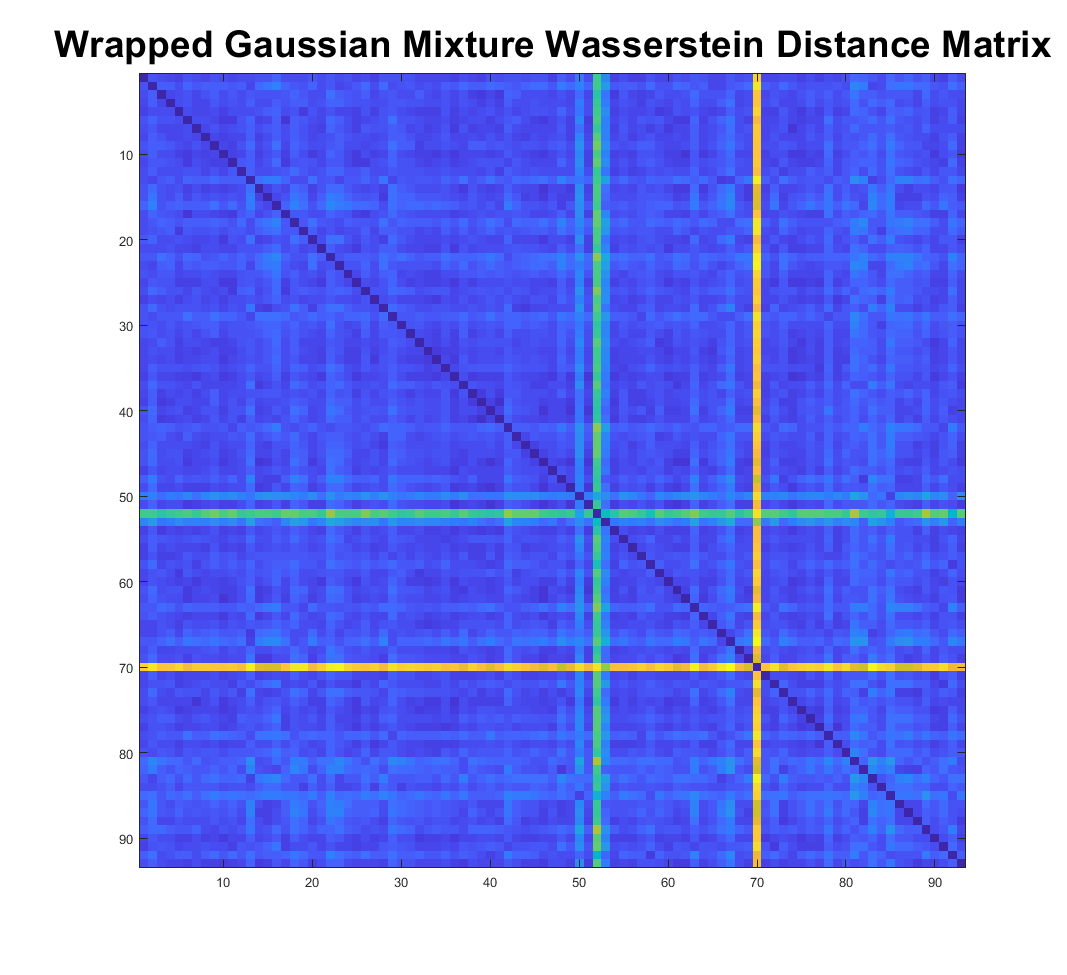
\includegraphics[width=.7\linewidth]{distance_matrix.png}
	\caption{Wrapped Gaussian Mixture Wasserstein-type Distance matrix. The first 42 columns/row correspond to non-PTSD subjects, columns/rows 43:93 correspond to PTSD subjects.  }
\end{center}
\end{figure}

One possible application of this approach is the comparison of the distributions of shapes, such as set of DTMRI fiber tracts. The data for this example consists of Fiber tractography data for the right Cingulum Parahippocampal region of 93 subjects in the Grady Trauma Project. 41 are diagnosed with PTSD, 42 are considered not to have PTSD. The regions are sets of fiber tracts, represented as curves in $\mathbb{R}^3$. We estimate these distributions by identifying shape modes in the shape space (using k-mode kernel mixture clustering) representing the distributions as Gaussian mixtures in the pre-shape space (which is a sphere) and then calculating the Wrapped Gaussian Mixture Wasserstein-type distance between the distributions of subjects. We then use these distances to classify subjects with respect to their PTSD status.

Specifically, let $X_i = \{ f_{ij}(t) \in L^2([0,1] \to \mathbb{R}^3), j = 1,...,M_j\}$, $i=1,...,93$ correspond to the set of fibers for subject $i$'s right Cingulum Parahippocampal region. For each $X_i$, we represent it as a wrapped Gaussian mixture $N(m_{ik}, \Sigma_{ik})$, where $m_k$ is the mode kth mode identified using the k-mode kernel mixture algorithm applied to the fibers for subject $i$, and $\Sigma_{ik}$ is the covariance of the fibers for subject $i$ assigned to cluster $k$, calculated in $T_{m_{ik}}(S^{d-1})$, the tangent space of the cluster mode in the pre-shape space. Using these as estimates for wrapped gaussian mixtures, we calculate Wasserstein-type distances using equation (\ref{eq: mixture distance}).       

The best classifier we found gets $\sim 60\%$ test set accuracy, which likely isn't significant. This could be because only a subset of mixture components is significant, causing the signal to get drowned out in the calculation of the Wasserstein distance, which takes comparisons of all mixture components down into a single number. 

\section{Conclusion}\label{section: conclusion}

\newpage

\bibliographystyle{plain}
\bibliography{refs} % Entries are in the refs.bib file

\cite{https://doi.org/10.48550/arxiv.1907.05254}
\cite{https://doi.org/10.48550/arxiv.0801.2250}
\cite{10.1307/mmj/1029003026}
\cite{COTFNT}
\cite{Ambrosio2013}
\cite{WGOT}


\end{document}

%\begin{equation}
%	W_2^2(\mu_0, \mu_1) =  \inf_{\gamma \in \gamma(\mu_0, \mu_1)} ||EX - EY|| + E||(X-EX)-(Y-EY)||  
%\end{equation}  
%
%\begin{equation}
%	= cos^{-1}(\langle m_0,m_1\rangle) + \inf_{\gamma \in \gamma(\mu_0, \mu_1)} \int_{S^{d-1} \times S^{d-1}} cos^{-1}(\langle Exp_{m_0}(R_\alpha(Exp_{m_1}^{-1}(y)), x)\rangle) \ d\gamma(x,y)
%\end{equation}
%
%\newpage

%\begin{equation}
%	= \inf_{\gamma \in \gamma(\mu_0, \mu_1)} \int_{\mathcal{X} \times \mathcal{Y}} ||x-y|| \ d\gamma(x,y) 
%\end{equation} 


%Now, since $cos^{-1}(\langle x,y \rangle) = ||Exp_{m_0}^{-1}(y) - Exp_{m_0}^{-1}(x)||$ and $R_\alpha(Exp_{m_1}^{-1}(y)) = Exp_{m_0}^{-1}(y) - Exp_{m_0}^{-1}(m_1)$, we have that
%
%\begin{equation}
%	cos^{-1}(\langle x,y \rangle) = ||R_\alpha(Exp_{m_1}^{-1}(y)) - Exp_{m_0}^{-1}(x) + Exp_{m_0}^{-1}(m_1)||
%\end{equation}
%
%Thus,
%
%\begin{equation}
%	\int_{S^{d-1} \times S^{d-1}} cos^{-1}(\langle x,y \rangle) d\gamma(x,y) = \int_{S^{d-1} \times S^{d-1}} ||R_\alpha(Exp_{m_1}^{-1}(y)) - Exp_{m_0}^{-1}(x) + Exp_{m_0}^{-1}(m_1)|| d\gamma(x,y)
%\end{equation}
%
%\begin{equation}
%	= \int_{S^{d-1} \times S^{d-1}} ||R_\alpha(Exp_{m_1}^{-1}(y)) - Exp_{m_0}^{-1}(x)\big)||  + \big\langle R_\alpha(Exp_{m_1}^{-1}(y)) - Exp_{m_0}^{-1}(x)), (Exp_{m_0}^{-1}(m_1)\big\rangle +  ||Exp_{m_0}^{-1}(m_1)|| d\gamma(x,y)
%\end{equation}
%
%\begin{multline}
%	= ||Exp_{m_0}^{-1}(m_1)||+ \int_{S^{d-1} \times S^{d-1}} ||R_\alpha(Exp_{m_1}^{-1}(y)) - Exp_{m_0}^{-1}(x)|| d\gamma(x,y) \\
%	+ \int_{S^{d-1} \times S^{d-1}} \big\langle R_\alpha(Exp_{m_1}^{-1}(y)) - Exp_{m_0}^{-1}(x)), (Exp_{m_0}^{-1}(m_1)\big\rangle d\gamma(x,y)
%\end{multline}
%
%\begin{equation}
% = cos^{-1}(\langle m_0,m_1\rangle) + \int_{S^{d-1} \times S^{d-1}} cos^{-1}(\langle Exp_{m_0}(R_\alpha(Exp_{m_1}^{-1}(y)), x)\rangle) \ d\gamma(x,y)
%\end{equation}
%
%
%
%\newpage

%
%\begin{equation}
%	= cos^{-1}(\langle m_0, m_1\rangle) + \inf_{\gamma \in \gamma(\mu_0, \mu_1)} \int_{S^{d-1} \times S^{d-1}} cos^{-1}(\big\langle x, f(y)\big \rangle) d\gamma(x,y) 
%\end{equation} 
%
%where $f(y) = Exp_{m_0} (R_\alpha( Exp_{m_1}^{-1}(y)))$, since
%
%\begin{equation}
%	R_\alpha(Exp_{m_1}^{-1}(y)) = Exp_{m_0}^{-1}(y) - Exp_{m_0}^{-1}(m_1)
%\end{equation}
%
%\begin{equation}
%	\implies ||Exp_{m_0}^{-1}(y) - Exp_{m_0}^{-1}(x) || = ||R_\alpha(Exp_{m_1}^{-1}(y)) - Exp_{m_0}^{-1}(x) + Exp_{m_0}^{-1}(m_1)||
%\end{equation}
%
%\begin{equation}
%	=  \Sigma_{i=1}^{d-1} (Exp_{m_0}^{-1}(y) - Exp_{m_0}^{-1}(x))^2 - 2(Exp_{m_0}^{-1}(y) - Exp_{m_0}^{-1}(x))(Exp_{m_0}^{-1}(m_1)) + (Exp_{m_0}^{-1}(m_1))^2 dy
%\end{equation}
%
%\begin{equation}
%	= cos^{-1}(\langle m_0,m_1\rangle) + cos^{-1}(\langle Exp_{m_0}(R_\alpha(Exp_{m_1}^{-1}(y)), Exp_{m_0}^{-1}(x))\rangle)
%\end{equation}



%Given $\mu_i = WN(m_i,\Sigma_i)$, $i = \{0,1\}$, where $m_i \in S_{d-1}$, and $\Sigma_i^{d-1 \times d-1}$, (and with densities $\rho_i$), the Wasserstein Distance between $\mu_0$ and $\mu_1$ can be calculated as;
%
%\begin{equation}\label{eq: wrapped normal wasserstein}
%	WNW_2^2(\mu_0, \mu_1) = cos^{-1}(\langle m_0, m_1 \rangle) + tr(\Sigma_0 + \Sigma_1 - 2(\Sigma_0^{\frac{1}{2}}\Sigma_1\Sigma_0^{\frac{1}{2}})^{\frac{1}{2}})
%\end{equation} 
%
%\textbf{Proof:}\\
%
%In order to prove this, we must find a continuous map $T:S^{d-1}\to S^{d-1}$ such that;
%
%1) $T$ pushes forward $\mu_0$ to $\mu_1$ ($\iff \rho_0(x) = \rho_1(Tx)|det T'|$)
%
%2) T is optimal 
%
%3) The transport cost of T is WNW\\

